\chapter{引言}

	\section{背景介绍}
    
        近年来, 云计算和移动计算获得了空前的发展, 面向服务的体系结构(SOA)已经成为了云计算和移动计算的主流架构\cite{wintergreen17}. 预计至2020年, SOA市场的规模将达到164亿美元. 而云计算业务的市场规模将于2021年达到715.5亿美元\cite{skyhighnetworks18azure}. 面向服务的体系结构经常使用web API的形式对外提供开放服务\cite{hamza15}, 这些web API常常使用SOAP(简单对象访问协议)协议或REST(表现层状态转换)风格\cite{fielding2000architectural}. Google云\cite{googlecloud17}, YouTube\cite{youtube17}, Amazon AWS\cite{amazonec217}和阿里云\cite{alibaba17}等等著名web应用均使用RESTful API作为服务接口. 一些大型公共API搜索引擎如APIs.io和百度API Store\footnote{到2017年, APIs.io(http://apis.io)数据库收录了1105项API, 而百度API Store(http://apistore.aidu.com)收录了1133项API.}均收录了超过1,000项面向web服务开发者的开放RESTful API. ProgrammableWeb平台\footnote{https://www.programmable.com/}可索引检索超过18,000项开放API.
        
        Web API常以公共服务的形式对外发布, 开发者则通过集成与组装这些web API的方法, 针对各种应用场景开发定制应用. 由于互联网应用环境的多样性和不可预测性, 在基于API的系统开发中, 缺陷和故障难以避免. API的开发者难以预见他们的API将会在什么用户场景下被用到, 更难以保证在这各种各样的环境下提供的API的绝对正确性. API的使用者也可能不熟悉API设计时对运行环境的限制, 进而很可能错误理解、错误使用这些API. 由于web API是这些上层应用的基础部件, 一旦某个web API被广泛应用, 它的任何疏漏和故障就会影响到众多应用和数以万计的用户, 甚至造成严重损失. 所以, web API的品质十分重要. 然而, web API的测试十分具有挑战性. 测试web API常常需要使用大量的测试用例来覆盖API的各种功能点和用法. 设计达到足够覆盖率的测试用例经常需要耗费大量的人力物力. 不仅如此, 由于web API实时提供、实时更新, 频繁的回归测试对于诊断和更新确认是必不可少的. 因此, 手动测试对于要求如此苛刻的web API连续集成测试而言, 是缺乏效率, 甚至是不适合采用的. web API的自动化测试, 从某种意义上, 已经成为了一种必需.

	\section{研究现状}
	
	    \label{sec:research_status}
	
    	结合本文的研究内容, 本文从三个方面考察了目前的研究现状: 领域专用语言与软件测试, 基于模型的测试, 和API自动化测试.
    	
    	在领域专用语言(Domain-Specific Language)和软件测试的结合方面, 有一些工作已经取得了一定的进展. Anurag Dwarakanath等人\cite{dwarakanatha17}设计了一种类似于英语的领域特定语言描述UI测试的测试用例. 该工作将UI测试的常见用户交互动作, 如鼠标点击, 屏幕滑动等, 形式化定义为语言中的语句, 在方便测试人员编写测试用例的同时又保证了机器可读性和定义严格性. Alex Gyori等人\cite{gyoria16}开发了NonDex工具, 对非形式化描述的Java API规范中的错误假设条件进行检测和修正. 他们的工作发现了Java标准库中一些API的实现对输入参数存在未写明的假设, 从侧面反映出API形式化定义的重要性. 在单API测试中, Andrea Arcuri\cite{andreaa17}应用遗传算法来为使用OpenAPI规约语言编写的RESTful API自动生成测试用例. OpenAPI\cite{openapi17}是一种描述RESTful web API行为的广受欢迎的领域专用语言, 我们的方法也基于OpenAPI. Ruben Verborgh和Michel Dumontier\cite{verborgh2016web}讨论了在基于功能的web API复用中, Swagger(OpenAPI的曾用名)规约语言脚本所起到的关键作用. Erik Wittern等人\cite{wittern2017statically}从GitHub中挖掘代码仓库, 然后基于OpenAPI语言的脚本自动检查JavaScript编写的API请求与标准的一致性. Swagger Inspector\cite{swaggerinspetor17}工具支持基于OpenAPI语言脚本的简单API测试, 但是多API的集成测试方面, 它仅仅支持发送单一序列请求, 能力尚有不足.
    	
    	基于模型的测试是测试自动化的重要研究方向. 近年来, 已经提出了许多模型和基于模型的软件测试技术. James A. Whittaker\cite{Whittaker1997}综述了马尔科夫模型及其随机性质在软件测试中的应用. Alan Jorgensen和James A. Whittaker\cite{jorgensen2000api}总结并提出了API测试的类型分区和马尔科夫建模测试法. 概率有限状态自动机(PFSA)\cite{enriquev05}是一种形式化定义的自动机模型, 它已经在软件建模和分析中得到了一定应用. 本文也将使用它作为场景模型的基础模型. Anand Raman和Jon Patrick\cite{anand97}提出了一种从序列分布中建模出对应PFSA模型的快速算法. 此算法扩展自一些更早期的工作, 如A. W. Biermann和J. A. Feldman提出的k-tails方法\cite{abiermann72}. 当使用本文的场景模型时, 可以应用此算法从用户调用历史数据中自动化构建使用场景模型. 而王钧奕等人\cite{junyiw17}在他们开发的分布式web API测试工具中使用了概率转移图模型. 此模型可以自动生成具有多样性的请求序列, 但是不能处理数据流的依赖, 约束和断言. Hung Viet Pham等人\cite{pham2016learning}提出了基于图的API调用场景表示和可从字节码中学习的API调用统计生成模型. 此外, Cyrille Artho等人\cite{cyrille17}在Apache ZooKeeper系统的API测试中使用了事件图模型. Robert Feldt和Simon Poulding\cite{feldt2017searching}总结出, 统计模型是一种生成特征多样化测试数据的重要方法.
    	
    	随着面向服务的体系架构和web API的日益流行, API的自动化测试日益成为研究热点. 在自动化生成API请求序列方面, 谢涛和裴健\cite{taox06}开发了MAPO工具, 此工具之后由钟浩进一步扩展\cite{Zhong2009}, 该工具融合了数据挖掘与代码分析方法, 可以挖掘API的频繁调用序列. 在此之后, Jaroslav Fowkes和Charles Sutton\cite{fowkes2016parameter}提出了PAM(概率式API挖掘器)算法, 这是一个几乎无需进行参数设置的API调用模式挖掘的概率式算法. 相比于MAPO, PAM在提取GitHub的相关API调用序列方面效果有明显提升. 循环神经网络(RNN)在序列建模方面十分有用. Junyoung Chung等人\cite{chung2014empirical}评估了很多不同类型的RNN单元在序列建模任务上的表现, 而API调用序列也是一类序列建模任务. 最近, 顾小东等人\cite{xiaodongg16}提出了一种用于API序列和依赖建模的基于RNN的自然语言模型. 在我们之前的工作中, 侯可佳等人\cite{kejiah13}分析了API序列的数据依赖和约束. 他们开发了进行自动化测试数据分区与生成的工具框架. 
    	
    	关于RESTful API的开发模式, Micheal Stowe\cite{michaels15}, Leonard Richardson和Sam Ruby\cite{leonardr07}讨论了规约驱动的RESTful API开发方式.
    	
    	Web API的场景模型, 在本文中主要用于自动化生成, 其实还可作为API用户的有效使用指南, 和API设计者的设计分析参考. Brad A. Myers等人\cite{bradm17}讨论了对API设计者, 开发者和用户而言, API易用性的含义和提高API易用性的重要性, 并提出了以用户需求分析为核心来提高API易用性的思想.

	\section{研究内容和结构安排}
	
	    本文的研究内容分为两大子课题: 场景建模与测试生成.
	
	    在场景建模方面, 本文提出了一种描述API使用场景的场景模型. 本文的场景模型对API服务的实际使用进行了抽象, 支持表达调用频率, 控制流依赖, 数据流依赖, 数据约束等等要素, 并讨论了场景模型的设计和生成.
	
        在测试生成方面, 本文主要提出了一种基于以上场景模型的web API自动化测试方法. 给出使用标准规约格式表达的场景模型, 本文提出的算法可以自动生成测试请求数据与测试执行序列, 实现复杂API组合测试的自动化.
        
        \begin{figure}[!htb]
            \centering
            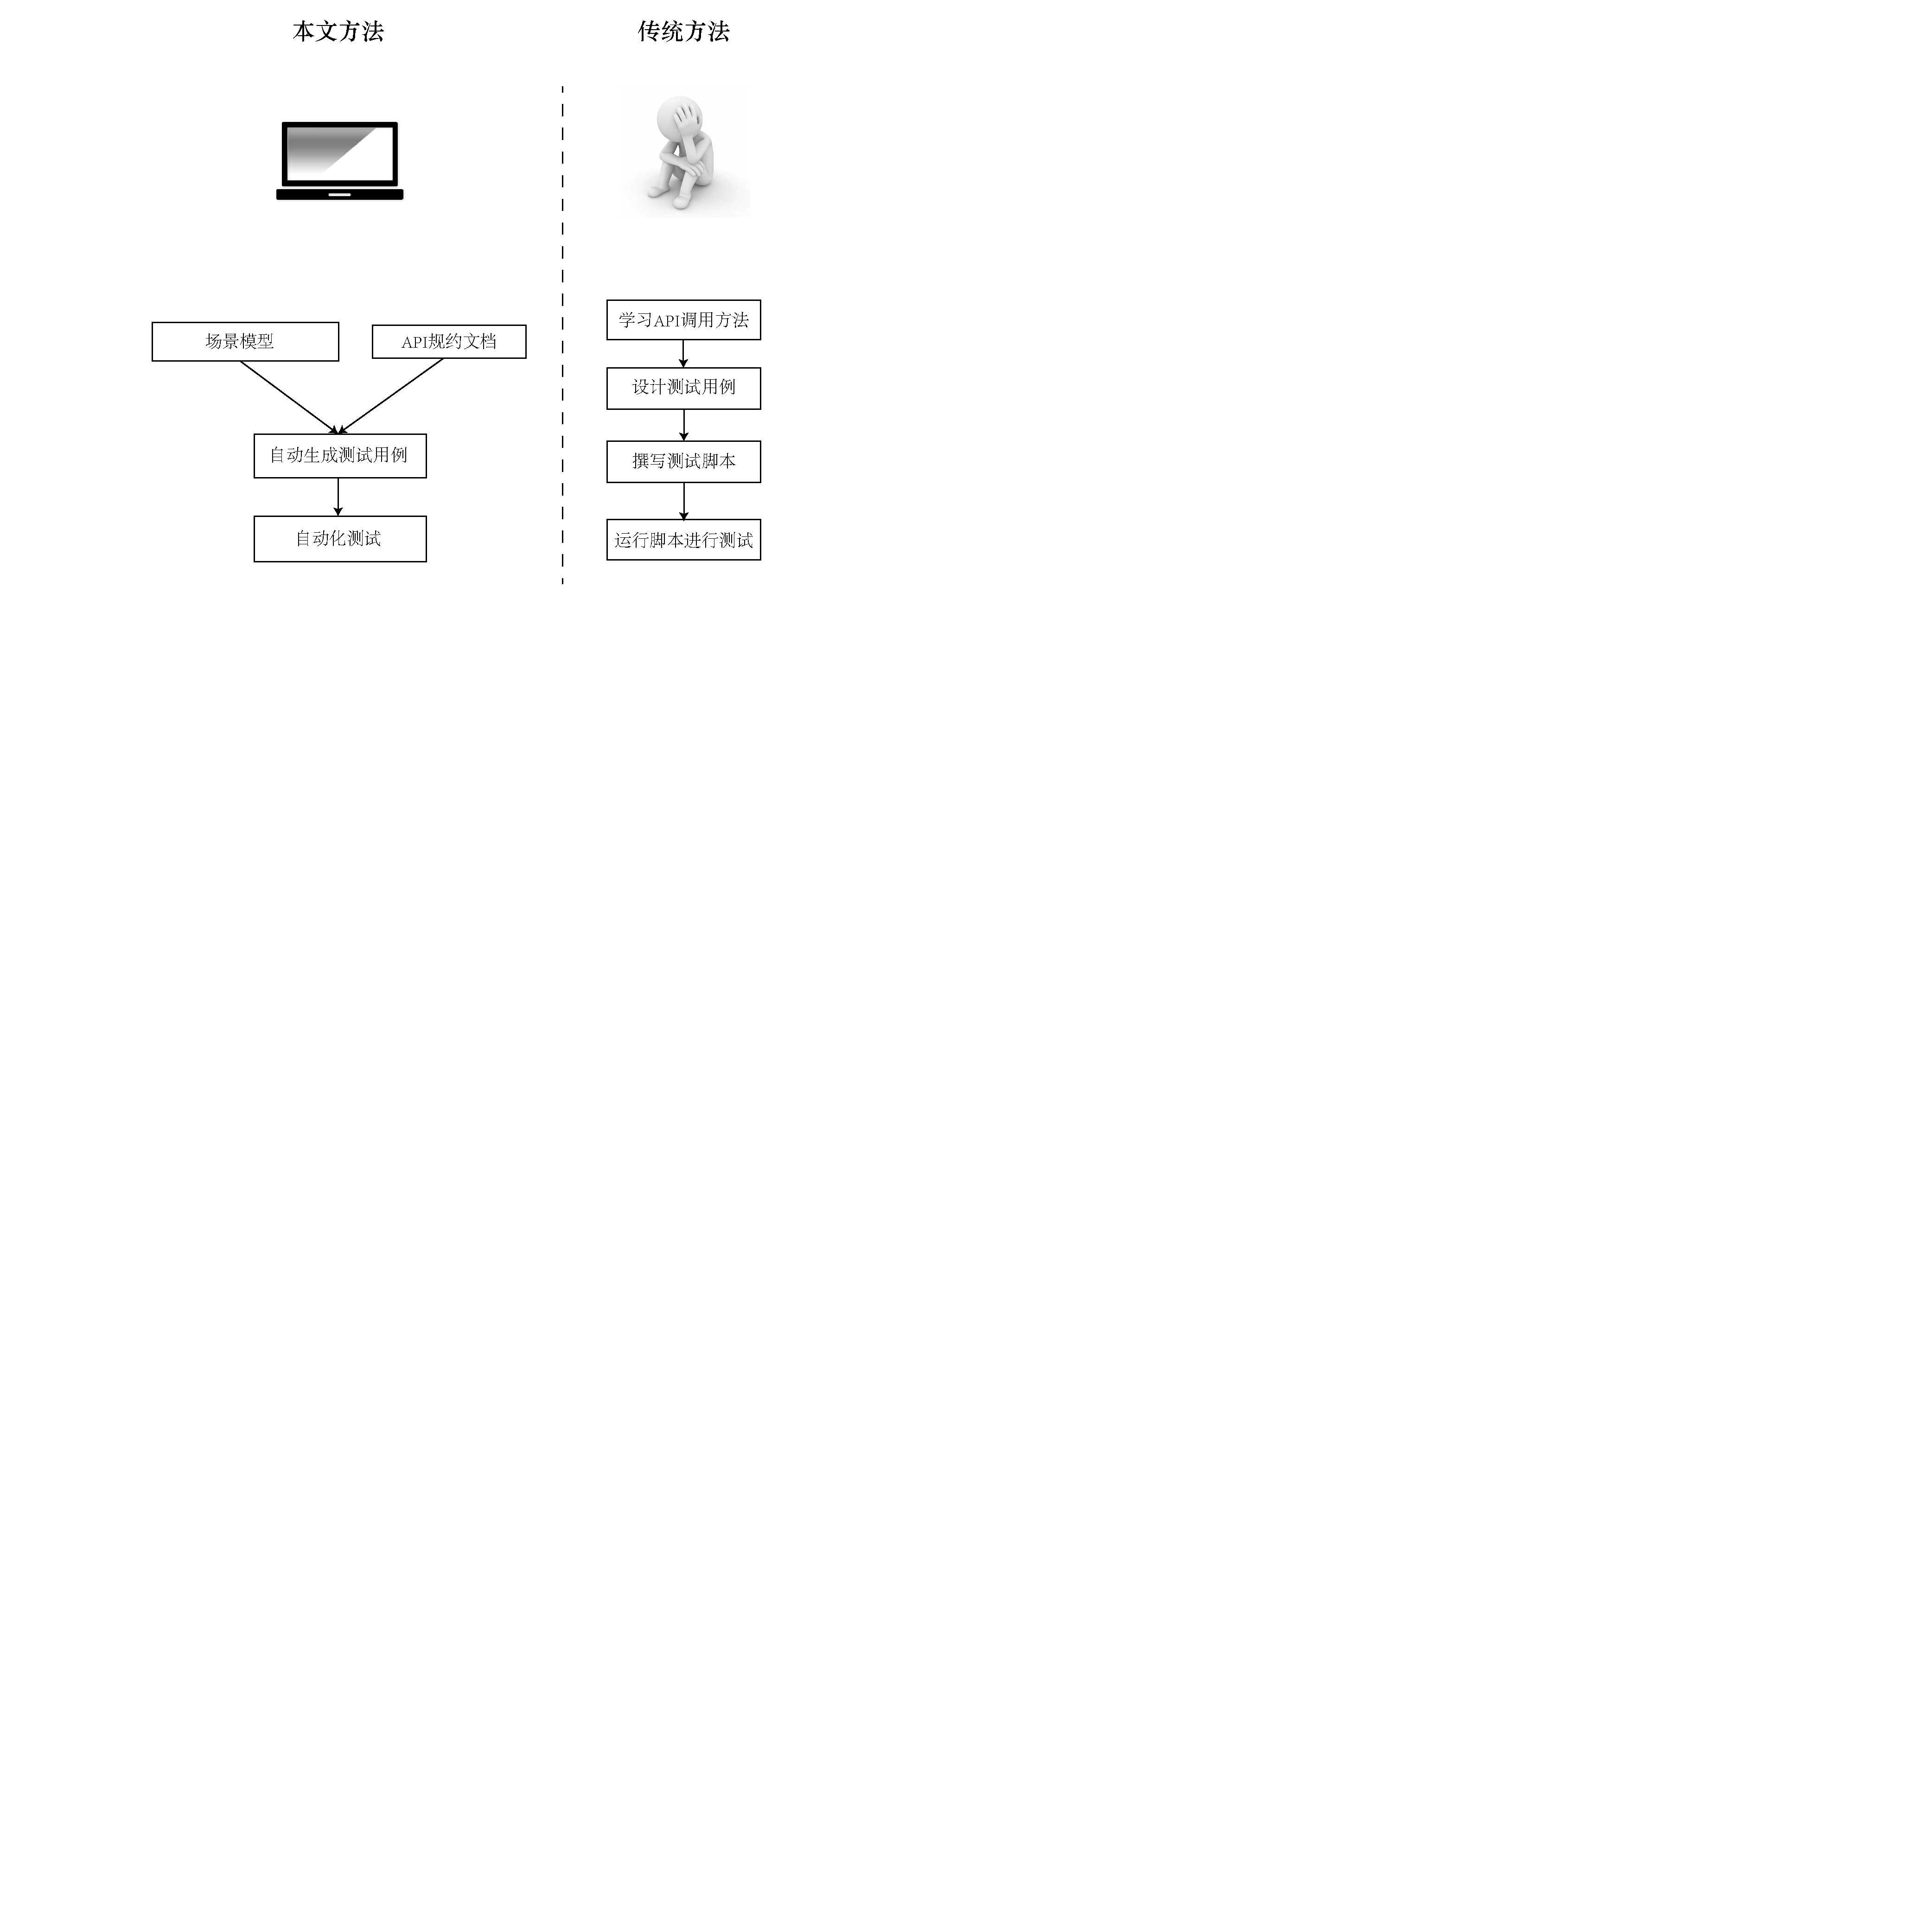
\includegraphics[width=400pt]{work_role_partial.pdf}
            \caption{本文方法与传统方法的对比. 在本文的方法中, 绝大多数环节均已完全自动化. 而在传统方法中, API调用方法的学习, 测试用例的设计, 以及测试脚本的编写等, 均需要大量人力付出.}
            \label{fig:overview}
        \end{figure}
        
        图\ref{fig:overview}展示了本文提出的自动化测试方法的总体框架, 并将其与传统人工方法进行了对比. 如图中右半部分所示, 在传统方法中, 人工测试员首先需要学习API的调用请求方法, 然后设计测试用例, 编写测试脚本, 并手动运行测试脚本. 这个过程需要大量的人力付出, 并且冗长无聊, 耗时耗力. 此外, 测试的质量还很大程度上依赖于测试员的经验和水平.
        
        为了应对这些困难, 本文提出的自动化测试方法相比于传统方法在以下方面进行了改进:
        \begin{itemize}
            \item 测试设计. \\
                在本文的方法中, 测试人员只需要手动或半自动地设计场景模型, 而不再是具体的每个测试用例. 本文的场景模型可以有效描述web API的控制流与数据流约束, 测试断言以及频繁使用模式. 相比直接设计测试用例, 由于一个测试场景可以自动生成多种各不相同的测试用例, 因此同样测试需求下, 所需场景数目少, 故设计测试场景可有效节约设计时间.
            
            \item 测试生成.\\
                在本文的方法中, 测试用例是由场景模型直接生成的. 使用本文提出的多种模块化测试数据生成算法和API调用序列生成算法, 测试用例的质量可以很容易地得到保证和提高. 并且, 由于实现了自动化, 测试用例的数量也可以远远超过手动设计的数量.
            
            \item 测试执行.\\
                目前已有的规约语言, 如OpenAPI, 提供了对RESTful API行为的详细形式化定义. 定义的组件包括了调用协议, 主机地址, 各个参数的格式和响应体的格式等等. 因此, 一旦有了测试数据, 便可以实现自动发送请求和响应解析.  本文实现了基于OpenAPI规约语言的工具原型, 可将人工测试员从书写API调用脚本的繁重劳动中解放出来.
        \end{itemize}
        
        本文实现了工具Lapis, 它完整实现了此自动化方法, 包括规约导向的API分析, 使用场景模型解析, 测试用例生成和测试用例执行等功能.
        
        本文的结构安排如下: 第一章总述研究的背景与现状. 第二章具体介绍场景模型. 第三章展开介绍基于场景模型进行自动化测试生成的方法, 并展示了方法在实际API服务上的实验结果. 第四章介绍工具的具体实现. 第五章进行总结, 并讨论了未来可继续进行的研究方向.
        
        % extended version
        % 本文的结构安排如下: 第二章介绍基本模型与方法, 包括形式化的场景模型, 和基于模型的测试数据与测试用例生成方法, 以及如何对生成的测试场景进行以故障检测为导向的优化. 第三章介绍原型系统的设计与实现, 包括原型系统的整体概述, 方法的具体实现等. 第四章展示原型系统在实际API服务上的实验结果, 并进行了实验结果的初步分析. 第五章进行总结, 并讨论了未来可继续进行的研究方向.
        

